% Options for packages loaded elsewhere
\PassOptionsToPackage{unicode}{hyperref}
\PassOptionsToPackage{hyphens}{url}
%
\documentclass[
]{book}
\usepackage{lmodern}
\usepackage{amssymb,amsmath}
\usepackage{ifxetex,ifluatex}
\ifnum 0\ifxetex 1\fi\ifluatex 1\fi=0 % if pdftex
  \usepackage[T1]{fontenc}
  \usepackage[utf8]{inputenc}
  \usepackage{textcomp} % provide euro and other symbols
\else % if luatex or xetex
  \usepackage{unicode-math}
  \defaultfontfeatures{Scale=MatchLowercase}
  \defaultfontfeatures[\rmfamily]{Ligatures=TeX,Scale=1}
\fi
% Use upquote if available, for straight quotes in verbatim environments
\IfFileExists{upquote.sty}{\usepackage{upquote}}{}
\IfFileExists{microtype.sty}{% use microtype if available
  \usepackage[]{microtype}
  \UseMicrotypeSet[protrusion]{basicmath} % disable protrusion for tt fonts
}{}
\makeatletter
\@ifundefined{KOMAClassName}{% if non-KOMA class
  \IfFileExists{parskip.sty}{%
    \usepackage{parskip}
  }{% else
    \setlength{\parindent}{0pt}
    \setlength{\parskip}{6pt plus 2pt minus 1pt}}
}{% if KOMA class
  \KOMAoptions{parskip=half}}
\makeatother
\usepackage{xcolor}
\IfFileExists{xurl.sty}{\usepackage{xurl}}{} % add URL line breaks if available
\IfFileExists{bookmark.sty}{\usepackage{bookmark}}{\usepackage{hyperref}}
\hypersetup{
  pdftitle={Data Science Course},
  pdfauthor={Fernando Racimo},
  hidelinks,
  pdfcreator={LaTeX via pandoc}}
\urlstyle{same} % disable monospaced font for URLs
\usepackage{color}
\usepackage{fancyvrb}
\newcommand{\VerbBar}{|}
\newcommand{\VERB}{\Verb[commandchars=\\\{\}]}
\DefineVerbatimEnvironment{Highlighting}{Verbatim}{commandchars=\\\{\}}
% Add ',fontsize=\small' for more characters per line
\usepackage{framed}
\definecolor{shadecolor}{RGB}{248,248,248}
\newenvironment{Shaded}{\begin{snugshade}}{\end{snugshade}}
\newcommand{\AlertTok}[1]{\textcolor[rgb]{0.94,0.16,0.16}{#1}}
\newcommand{\AnnotationTok}[1]{\textcolor[rgb]{0.56,0.35,0.01}{\textbf{\textit{#1}}}}
\newcommand{\AttributeTok}[1]{\textcolor[rgb]{0.77,0.63,0.00}{#1}}
\newcommand{\BaseNTok}[1]{\textcolor[rgb]{0.00,0.00,0.81}{#1}}
\newcommand{\BuiltInTok}[1]{#1}
\newcommand{\CharTok}[1]{\textcolor[rgb]{0.31,0.60,0.02}{#1}}
\newcommand{\CommentTok}[1]{\textcolor[rgb]{0.56,0.35,0.01}{\textit{#1}}}
\newcommand{\CommentVarTok}[1]{\textcolor[rgb]{0.56,0.35,0.01}{\textbf{\textit{#1}}}}
\newcommand{\ConstantTok}[1]{\textcolor[rgb]{0.00,0.00,0.00}{#1}}
\newcommand{\ControlFlowTok}[1]{\textcolor[rgb]{0.13,0.29,0.53}{\textbf{#1}}}
\newcommand{\DataTypeTok}[1]{\textcolor[rgb]{0.13,0.29,0.53}{#1}}
\newcommand{\DecValTok}[1]{\textcolor[rgb]{0.00,0.00,0.81}{#1}}
\newcommand{\DocumentationTok}[1]{\textcolor[rgb]{0.56,0.35,0.01}{\textbf{\textit{#1}}}}
\newcommand{\ErrorTok}[1]{\textcolor[rgb]{0.64,0.00,0.00}{\textbf{#1}}}
\newcommand{\ExtensionTok}[1]{#1}
\newcommand{\FloatTok}[1]{\textcolor[rgb]{0.00,0.00,0.81}{#1}}
\newcommand{\FunctionTok}[1]{\textcolor[rgb]{0.00,0.00,0.00}{#1}}
\newcommand{\ImportTok}[1]{#1}
\newcommand{\InformationTok}[1]{\textcolor[rgb]{0.56,0.35,0.01}{\textbf{\textit{#1}}}}
\newcommand{\KeywordTok}[1]{\textcolor[rgb]{0.13,0.29,0.53}{\textbf{#1}}}
\newcommand{\NormalTok}[1]{#1}
\newcommand{\OperatorTok}[1]{\textcolor[rgb]{0.81,0.36,0.00}{\textbf{#1}}}
\newcommand{\OtherTok}[1]{\textcolor[rgb]{0.56,0.35,0.01}{#1}}
\newcommand{\PreprocessorTok}[1]{\textcolor[rgb]{0.56,0.35,0.01}{\textit{#1}}}
\newcommand{\RegionMarkerTok}[1]{#1}
\newcommand{\SpecialCharTok}[1]{\textcolor[rgb]{0.00,0.00,0.00}{#1}}
\newcommand{\SpecialStringTok}[1]{\textcolor[rgb]{0.31,0.60,0.02}{#1}}
\newcommand{\StringTok}[1]{\textcolor[rgb]{0.31,0.60,0.02}{#1}}
\newcommand{\VariableTok}[1]{\textcolor[rgb]{0.00,0.00,0.00}{#1}}
\newcommand{\VerbatimStringTok}[1]{\textcolor[rgb]{0.31,0.60,0.02}{#1}}
\newcommand{\WarningTok}[1]{\textcolor[rgb]{0.56,0.35,0.01}{\textbf{\textit{#1}}}}
\usepackage{longtable,booktabs}
% Correct order of tables after \paragraph or \subparagraph
\usepackage{etoolbox}
\makeatletter
\patchcmd\longtable{\par}{\if@noskipsec\mbox{}\fi\par}{}{}
\makeatother
% Allow footnotes in longtable head/foot
\IfFileExists{footnotehyper.sty}{\usepackage{footnotehyper}}{\usepackage{footnote}}
\makesavenoteenv{longtable}
\usepackage{graphicx}
\makeatletter
\def\maxwidth{\ifdim\Gin@nat@width>\linewidth\linewidth\else\Gin@nat@width\fi}
\def\maxheight{\ifdim\Gin@nat@height>\textheight\textheight\else\Gin@nat@height\fi}
\makeatother
% Scale images if necessary, so that they will not overflow the page
% margins by default, and it is still possible to overwrite the defaults
% using explicit options in \includegraphics[width, height, ...]{}
\setkeys{Gin}{width=\maxwidth,height=\maxheight,keepaspectratio}
% Set default figure placement to htbp
\makeatletter
\def\fps@figure{htbp}
\makeatother
\setlength{\emergencystretch}{3em} % prevent overfull lines
\providecommand{\tightlist}{%
  \setlength{\itemsep}{0pt}\setlength{\parskip}{0pt}}
\setcounter{secnumdepth}{5}
\usepackage{booktabs}
\ifluatex
  \usepackage{selnolig}  % disable illegal ligatures
\fi
\usepackage[]{natbib}
\bibliographystyle{apalike}

\title{Data Science Course}
\author{Fernando Racimo}
\date{2020-10-17}

\begin{document}
\maketitle

{
\setcounter{tocdepth}{1}
\tableofcontents
}
\hypertarget{introduction}{%
\chapter{Introduction}\label{introduction}}

To compile this example to PDF, you need XeLaTeX. You are recommended to install TinyTeX (which includes XeLaTeX): \url{https://yihui.org/tinytex/}.

\hypertarget{intro}{%
\chapter{Getting Started with Data Analysis}\label{intro}}

You can label chapter and section titles using \texttt{\{\#label\}} after them, e.g., we can reference Chapter \ref{intro}. If you do not manually label them, there will be automatic labels anyway, e.g., Chapter \ref{methods}.

Figures and tables with captions will be placed in \texttt{figure} and \texttt{table} environments, respectively.

\begin{Shaded}
\begin{Highlighting}[]
\KeywordTok{par}\NormalTok{(}\DataTypeTok{mar =} \KeywordTok{c}\NormalTok{(}\DecValTok{4}\NormalTok{, }\DecValTok{4}\NormalTok{, }\FloatTok{.1}\NormalTok{, }\FloatTok{.1}\NormalTok{))}
\KeywordTok{plot}\NormalTok{(pressure, }\DataTypeTok{type =} \StringTok{\textquotesingle{}b\textquotesingle{}}\NormalTok{, }\DataTypeTok{pch =} \DecValTok{19}\NormalTok{)}
\end{Highlighting}
\end{Shaded}

\begin{figure}

{\centering 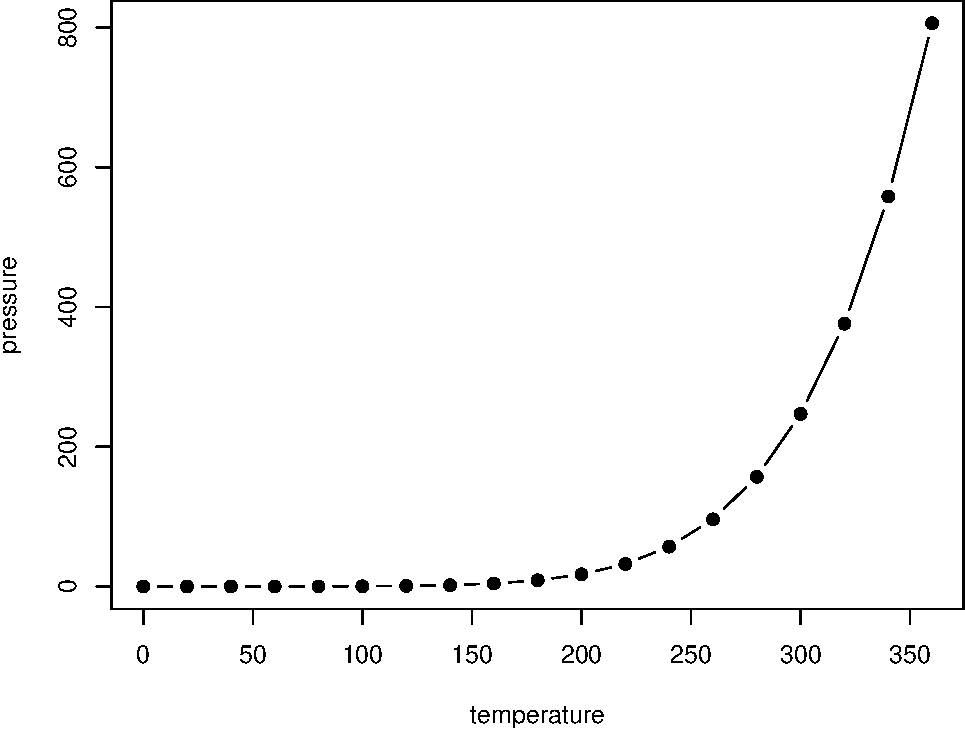
\includegraphics[width=0.8\linewidth]{DataScience_files/figure-latex/nice-fig-1} 

}

\caption{Here is a nice figure!}\label{fig:nice-fig}
\end{figure}

Reference a figure by its code chunk label with the \texttt{fig:} prefix, e.g., see Figure \ref{fig:nice-fig}. Similarly, you can reference tables generated from \texttt{knitr::kable()}, e.g., see Table \ref{tab:nice-tab}.

\begin{Shaded}
\begin{Highlighting}[]
\NormalTok{knitr}\OperatorTok{::}\KeywordTok{kable}\NormalTok{(}
  \KeywordTok{head}\NormalTok{(iris, }\DecValTok{20}\NormalTok{), }\DataTypeTok{caption =} \StringTok{\textquotesingle{}Here is a nice table!\textquotesingle{}}\NormalTok{,}
  \DataTypeTok{booktabs =} \OtherTok{TRUE}
\NormalTok{)}
\end{Highlighting}
\end{Shaded}

\begin{table}

\caption{\label{tab:nice-tab}Here is a nice table!}
\centering
\begin{tabular}[t]{rrrrl}
\toprule
Sepal.Length & Sepal.Width & Petal.Length & Petal.Width & Species\\
\midrule
5.1 & 3.5 & 1.4 & 0.2 & setosa\\
4.9 & 3.0 & 1.4 & 0.2 & setosa\\
4.7 & 3.2 & 1.3 & 0.2 & setosa\\
4.6 & 3.1 & 1.5 & 0.2 & setosa\\
5.0 & 3.6 & 1.4 & 0.2 & setosa\\
\addlinespace
5.4 & 3.9 & 1.7 & 0.4 & setosa\\
4.6 & 3.4 & 1.4 & 0.3 & setosa\\
5.0 & 3.4 & 1.5 & 0.2 & setosa\\
4.4 & 2.9 & 1.4 & 0.2 & setosa\\
4.9 & 3.1 & 1.5 & 0.1 & setosa\\
\addlinespace
5.4 & 3.7 & 1.5 & 0.2 & setosa\\
4.8 & 3.4 & 1.6 & 0.2 & setosa\\
4.8 & 3.0 & 1.4 & 0.1 & setosa\\
4.3 & 3.0 & 1.1 & 0.1 & setosa\\
5.8 & 4.0 & 1.2 & 0.2 & setosa\\
\addlinespace
5.7 & 4.4 & 1.5 & 0.4 & setosa\\
5.4 & 3.9 & 1.3 & 0.4 & setosa\\
5.1 & 3.5 & 1.4 & 0.3 & setosa\\
5.7 & 3.8 & 1.7 & 0.3 & setosa\\
5.1 & 3.8 & 1.5 & 0.3 & setosa\\
\bottomrule
\end{tabular}
\end{table}

You can write citations, too. For example, we are using the \textbf{bookdown} package \citep{R-bookdown} in this sample book, which was built on top of R Markdown and \textbf{knitr} \citep{xie2015}.

\hypertarget{prob}{%
\chapter{Probability}\label{prob}}

\hypertarget{tossing-a-coin-the-bernoulli-distribution}{%
\section{Tossing a coin: the Bernoulli distribution}\label{tossing-a-coin-the-bernoulli-distribution}}

We can ``virtually'' toss a coin in our R console, using the rbinom() function:

\begin{Shaded}
\begin{Highlighting}[]
\KeywordTok{rbinom}\NormalTok{(}\DecValTok{1}\NormalTok{, }\DecValTok{1}\NormalTok{,.}\DecValTok{5}\NormalTok{)}
\end{Highlighting}
\end{Shaded}

\begin{verbatim}
## [1] 1
\end{verbatim}

Try copying the above chunk to your R console and running it multiple times. Do you always get the same result?

This function has 3 required input parameters: n, size and prob. The first parameter (n) determines the number of trials we are telling R to perform, in other words, the number of coin tosses we want to generate:

\begin{Shaded}
\begin{Highlighting}[]
\KeywordTok{rbinom}\NormalTok{(}\DecValTok{20}\NormalTok{, }\DecValTok{1}\NormalTok{,}\FloatTok{0.5}\NormalTok{)}
\end{Highlighting}
\end{Shaded}

\begin{verbatim}
##  [1] 1 0 1 0 1 0 0 1 0 0 1 1 0 1 1 0 0 1 1 1
\end{verbatim}

Here, we generate 20 toin cosses, and the zeroes and ones represent whether we got a heads or a tails in each trial. For now, we will ignore the second parameter (size) and fitted it at 1, but we'll revisit it in a moment. The third parameter (prob) dictates how biased the coin is. If we set it to 0.9, we'll get the outcomes of a biased coin toss, in particular biased towards heads:

\begin{Shaded}
\begin{Highlighting}[]
\KeywordTok{rbinom}\NormalTok{(}\DecValTok{20}\NormalTok{, }\DecValTok{1}\NormalTok{,}\FloatTok{0.9}\NormalTok{)}
\end{Highlighting}
\end{Shaded}

\begin{verbatim}
##  [1] 1 1 1 1 1 1 1 1 1 0 1 1 1 1 1 0 1 1 1 1
\end{verbatim}

What happens when you set prob to 0.1? Or 0.999? Why?

What we are really doing here is simulating outcomes of a random variable that is governed by a particular probability distribution (in this case, the Bernoulli distribution). We can assign a name to this variable for storage and manipulation later on:

\begin{Shaded}
\begin{Highlighting}[]
\NormalTok{X \textless{}{-}}\StringTok{ }\KeywordTok{rbinom}\NormalTok{(}\DecValTok{1}\NormalTok{, }\DecValTok{1}\NormalTok{,}\FloatTok{0.9}\NormalTok{)}
\end{Highlighting}
\end{Shaded}

If you type this in your console, X will now store the value of the outcome of a biased coin toss (either 0 or 1), which you can use later in your code.

How can we verify that R is really doing what we think it is doing? Well, if we think we have a fair coin and we throw it many times, then, on average, we should get the same number of heads and tails, right? This experiment should be more accurate the more trials we have. We can compute the average of our coin tosses by using the function sum(), which adds the elements of a vector, and then dividing by the total number of trials.

Let's create a new variable (n) that will determine how many trials we attempt, say 20.

\begin{Shaded}
\begin{Highlighting}[]
\NormalTok{n \textless{}{-}}\StringTok{ }\DecValTok{20}
\KeywordTok{sum}\NormalTok{(}\KeywordTok{rbinom}\NormalTok{(n,}\DecValTok{1}\NormalTok{,}\FloatTok{0.5}\NormalTok{)) }\OperatorTok{/}\StringTok{ }\NormalTok{n}
\end{Highlighting}
\end{Shaded}

\begin{verbatim}
## [1] 0.35
\end{verbatim}

Try copying this into your console. Do you get the same number as I do? Do you get exactly 0.5? If not, why not? Try the same exercise but with 100 trials, 1000 trials and 100000 trials. What happens as we increase the number of trials?

This should illustrate how powerful R can be. We just threw 100 thousand coins into the air without even lifting our fingers! Try to repeat the exercise above, but this time, set the Bernoulli prob parameter to be equal to a number of your choice (between 0 and 1). What is the average of all your coin tosses?

\hypertarget{adding-up-many-coin-tosses-the-binomial-distribution}{%
\section{Adding up many coin tosses: the Binomial distribution}\label{adding-up-many-coin-tosses-the-binomial-distribution}}

Let's say we are now not interested in any particular coin toss, but in the sum of our coin tosses. Each toss is represented by a 0 or a 1, so the sum of all our tosses cannot be smaller than 0 or larger than the total number of tosses we perform.

Try running the below code 5 times. What numbers do you obtain?

\begin{Shaded}
\begin{Highlighting}[]
\KeywordTok{sum}\NormalTok{(}\KeywordTok{rbinom}\NormalTok{(}\DecValTok{20}\NormalTok{,}\DecValTok{1}\NormalTok{,}\FloatTok{0.5}\NormalTok{))}
\end{Highlighting}
\end{Shaded}

\begin{verbatim}
## [1] 7
\end{verbatim}

Turns out there's a short-hand way of performing the same experiment, i.e.~tossing a bunch of coins - each a Bernoulli random variable - observing their outcomes and adding them up, without using the sum() function at all. Here's where the second input parameter - size - of the rbinom() function comes into play. So far, we've always left it equal to 1 in all our command lines above, but we can set it to any positive integer:

\begin{Shaded}
\begin{Highlighting}[]
\KeywordTok{rbinom}\NormalTok{(}\DecValTok{1}\NormalTok{,}\DecValTok{20}\NormalTok{,}\FloatTok{0.5}\NormalTok{)}
\end{Highlighting}
\end{Shaded}

\begin{verbatim}
## [1] 12
\end{verbatim}

The above code is equivalent to taking 20 Bernoulli trials, and then adding their outcomes up. The ``experiment'' we are running is now not a single coin toss, but 20 coin tosses together. The outcome of this experiment is neither heads nor tails, but the sum of all the heads in all those coin tosses. It turns out that this ``experiment'' is a probability distribution in its own right, and it is called the Binomial distribution. It has two parameters: the size of the experiment (how many tosses we perform) and the probability of heads for each toss (the prob parameter). The Bernoulli distribution is just a specific case of the Binomial distribution (the case in which we only toss 1 coin, i.e.~size = 1). You can read more about this distribution if you go to the help menu for this function (type "?rbinom).

\hypertarget{the-expectation-of-a-random-variable}{%
\section{The expectation of a random variable}\label{the-expectation-of-a-random-variable}}

We can take the average of multiple Binomial trials as well. Let's try adding the results of 5 Binomial trials, each with size 20 (how many Bernoulli trials is this equivalent to?):

\begin{Shaded}
\begin{Highlighting}[]
\NormalTok{n \textless{}{-}}\StringTok{ }\DecValTok{5}
\NormalTok{size \textless{}{-}}\StringTok{ }\DecValTok{20}
\NormalTok{prob \textless{}{-}}\StringTok{ }\FloatTok{0.5}
\NormalTok{X \textless{}{-}}\StringTok{ }\KeywordTok{rbinom}\NormalTok{(n,size,prob)}
\NormalTok{X}
\end{Highlighting}
\end{Shaded}

\begin{verbatim}
## [1] 13  9  9 10  8
\end{verbatim}

\begin{Shaded}
\begin{Highlighting}[]
\NormalTok{Xsum \textless{}{-}}\StringTok{ }\KeywordTok{sum}\NormalTok{(X)}
\NormalTok{Xsum}
\end{Highlighting}
\end{Shaded}

\begin{verbatim}
## [1] 49
\end{verbatim}

To get the average, we divide by the total number of trials (remember here that the number of Binomial trials is 5):

\begin{Shaded}
\begin{Highlighting}[]
\NormalTok{Xave \textless{}{-}}\StringTok{ }\NormalTok{Xsum }\OperatorTok{/}\StringTok{ }\NormalTok{n}
\NormalTok{Xave}
\end{Highlighting}
\end{Shaded}

\begin{verbatim}
## [1] 9.8
\end{verbatim}

A shorthand for obtaining the mean is the function mean(). This should give you the same result:

\begin{Shaded}
\begin{Highlighting}[]
\NormalTok{Xave \textless{}{-}}\StringTok{ }\KeywordTok{mean}\NormalTok{(X)}
\NormalTok{Xave}
\end{Highlighting}
\end{Shaded}

\begin{verbatim}
## [1] 9.8
\end{verbatim}

Note that the mean need not be an integer, even if each Binomial trial \emph{must} be an integer.

Now, try repeating the same exercise but using 100 Binomial trials, and then 100 thousand Binomial trials. What numbers do you get? What number do we expect to get as we increase the number of Binomial trials?

This number is called the \emph{Expectation} of a random variable. It is defined as follows:

\[E[X] = \sum_{i}x_iP[X=x_i]\]

Here the sum is over all possible values that the random variable X can take. In other words, it is equal to the sum of each of these values, weighted by the probability that the random variable takes that value.

In the case of a variable that follows the Binomial distribution, the expectation happens to be equal to the product of size and prob:

\[E[X] = n * p\]

(note that the n here refers to the size of a single Binomial trial).

This should make intuitive sense: if we throw a bunch of coins and add up their results, the number we expect to get should be approximately equal to the probability of heads times the number of tosses we perform. Note that this equality only holds approximately: for any given Binomial trial, we can get any number between 0 and the size of the Binomial experiment. If we take an average over many Binomial experiments, we'll approach this expectation ever more accurately. The average (also called ``sample mean'' ) over a series of experiments is thus an approximation to the expectation, which is often unknown in real life. The sample mean is often represented by a letter with a bar on top: \[\bar{x} = \frac{\sum_{i}^{n}x_{i}}{n}\]

You can think of the expectation as the mean over an infinite number of trials.

\hypertarget{our-first-probability-mass-function}{%
\section{Our first probability mass function}\label{our-first-probability-mass-function}}

Ok, all this talk of Bernoulli and Binomial is great. But what is the point of it? The nice thing about probability theory is that it allows us to better think about processes in nature, by codifying these processes into mathematical equations.

For example, going back to our coin tossing example, if someone asked you how many heads you'd expect among 20 tosses, your best bet would be to give the mean of a Binomial distribution with size 20 and probability of heads equal to 0.5: \[0.5*20=10\].

But this is a fairly intuitive answer. You didn't need probability theory to tell you that about half the coins would turn out heads. Plus, we all know that one might not get 10 heads (we might get 9, 13 or even 0 if we're very unlucky). What is then, the probability that we would get 10 heads? In other words, if we were to repeat our Binomial experiment of 20 tosses a large number of times, how many of those experiments would yield exactly 10 heads? This is a much harder question to answer. Do you have a guess?

It turns out that probability theory can come to the rescue. The Binomial distribution has a very neat equation called its ``Probability Mass Function'', which answers this question exactly:

\[P[ X = k ] = {n \choose k}p^{k}(1-p)^{n-k}\]

If we let k = 10, and plug in our values for the sample size and probability of heads, we get an exact answer:

\[P[ X = 10 ] = {20 \choose 10}0.5^{10}0.5^{10} = 0.1762...\]

So in about 17\% of experiments, we should get 10 heads out of the 20 tosses.

Let's unpack this equation a bit. You can see that it has 3 terms, which are multiplied together. We'll ignore the first term for now. Let's focus on the second term: \(p^{k}\). This is simply equivalent to multiplying our probability of heads k times. In other words, this means that we need k of the tosses to be heads, and the probability of this happening is just the product of the probability of heads in each of the total (n) tosses. In our case, \(k=10\), because we need 10 tosses, and \(n=20\) because we tossed the coin 20 times. So far, so good.

The third term is very similar. We not only need 10 heads, but also 10 tails (because we need exactly 10 of the tosses to be heads, no more, no less). The probability of this happening is the product of the probability of getting tails \((1-p)\) multiplied \(n-k\) times. In our case, \(n-k\) happens to also be equal to 10.

But what about the first term: \(n \choose k\) ? This is called a binomial coefficient. It is used to represent the ways in which one can choose an unordered subset of k elements from a fixed set of n elements. In our case, we need 10 of our 20 tosses to be heads, but we don't need to specify exactly which of the tosses will be heads. It could be that we head 10 heads followed by 10 tails, or 1 head and 1 tail one after the other, or any arbitrary combination of 10 heads and 10 tails. The binomial coefficient gives us the number of all these combinations. It is defined as:

\[{n \choose k} = \frac{n!}{k!(n-k)!}\]

where

\[a! = a(a-1)(a-2)(a-3) ...1\]
Try plugging in other values of k into the Probability Mass Function (PMF) of the Binomial distribution. What probabilities do you get? How do these change as the numbers are closer or farther away from the expectation (\(n*p=10\))?

Ok, this is very neat, but how can we check this equation is correct? Well, we can use simulations! In other words, we can generate a large number of Binomial trials, and check how many of those are exactly equal to our choice of k. This fraction of all trials should approximate \(P[X=k]\). Let's try this for \(k=10\) and 500 trials.

\begin{Shaded}
\begin{Highlighting}[]
\NormalTok{n \textless{}{-}}\StringTok{ }\DecValTok{500}
\NormalTok{size \textless{}{-}}\StringTok{ }\DecValTok{20}
\NormalTok{prob \textless{}{-}}\StringTok{ }\FloatTok{0.5}
\NormalTok{X \textless{}{-}}\StringTok{ }\KeywordTok{rbinom}\NormalTok{(n,size,prob)}
\NormalTok{X}
\end{Highlighting}
\end{Shaded}

\begin{verbatim}
##   [1]  9  8 10 12  8 10 15 10  9  9 10  8 13  8 13 12  7 10  9 10  8 11 12  6  7
##  [26] 10  7  8  8  9  9 13 11  8 11 11 12 13 10  5 10  8 13  8 13  9 11 11  8 11
##  [51] 10 10 10 12 11 11 10 15  7 13 12 11 10 10 10 10 10 11 11  8 10 12  9 11 10
##  [76] 11  9 10  8  9 12  8  5 13  8 11 11 13 11 10 11 11 14  9  9 13 13 13  6 11
## [101] 12  5 10 11 11  6  8 10 13  8  9 10  6 10  8 10  9  6 13 12  8 14  6  7 14
## [126] 13  9  9  9 10 11  9  9  9 12 10 11 10 11  8  8  8 13  9  9 12 10 13  8  4
## [151] 11 14  9 12  4 14  9 11  9  9 11 10 11 10 13 11  8  9 13  9  6 12 11 12 10
## [176] 10  8 10 13 10 11  8  8  5 12 11 13 12 11  9 12  7 11 12 12 10  8 10 10  7
## [201]  9  7  8 10 10 10  9  9 10 11  7 10  8  9  8  9  9  7  9 10  9  8 10 10 10
## [226] 12 10 10 12 14 11 10  9 10 11 10 13 13  8 10 15 11 11 10  9  9  9 13 10 11
## [251]  9  6 13  8  8 12 13 10 12 11  9 10  9 11 13  7 11  6  7 10  6  9  9 10  8
## [276] 10 12 12 10  9 12 13 16  9 11 16  8 10  9  6 13 15 10 12  9  9 14 12 11 14
## [301] 12  5  9 11  6 10 12 13 10 12 10 12 12 10 13 10  9  6 13  8 12  6 12  7  7
## [326] 11 13  7  9  7 12  7  8  9  9 13  8 11 14  9  9 13  9  9  8  9 12 11 10 13
## [351] 10  8 10  9  7 11  8 10  8  6  7  6 13  6  8  7 11 12 12 10 13 10 12 10 13
## [376] 10 13  9  9  8 10 14 13  8 16 10 10 13 12 12  6  9 13 11 10  8  8 11  9 10
## [401]  9 10 11  8 12 11 10  9 11 11  8 15 12  7  7 12  6 10 13  7 10 10  9 13  9
## [426] 12 11 15  8 10 11 11  7  9  9  8 11 13 12 10  9  9 11  9 12 10 12  9  4  7
## [451]  8 10  8 14  8 10 10 13 14 12 11 13 10 12 13  6 11  8  8  9 11 11  9  9  5
## [476] 14 11 14  8 11 10  8  8 11 12 10 11  9 10  9 11 12 11  6 12 15  9 11 10  8
\end{verbatim}

We can determine which of these trials was equal to 10:

\begin{Shaded}
\begin{Highlighting}[]
\NormalTok{verify \textless{}{-}}\StringTok{ }\NormalTok{(X }\OperatorTok{==}\StringTok{ }\DecValTok{10}\NormalTok{)}
\NormalTok{verify}
\end{Highlighting}
\end{Shaded}

\begin{verbatim}
##   [1] FALSE FALSE  TRUE FALSE FALSE  TRUE FALSE  TRUE FALSE FALSE  TRUE FALSE
##  [13] FALSE FALSE FALSE FALSE FALSE  TRUE FALSE  TRUE FALSE FALSE FALSE FALSE
##  [25] FALSE  TRUE FALSE FALSE FALSE FALSE FALSE FALSE FALSE FALSE FALSE FALSE
##  [37] FALSE FALSE  TRUE FALSE  TRUE FALSE FALSE FALSE FALSE FALSE FALSE FALSE
##  [49] FALSE FALSE  TRUE  TRUE  TRUE FALSE FALSE FALSE  TRUE FALSE FALSE FALSE
##  [61] FALSE FALSE  TRUE  TRUE  TRUE  TRUE  TRUE FALSE FALSE FALSE  TRUE FALSE
##  [73] FALSE FALSE  TRUE FALSE FALSE  TRUE FALSE FALSE FALSE FALSE FALSE FALSE
##  [85] FALSE FALSE FALSE FALSE FALSE  TRUE FALSE FALSE FALSE FALSE FALSE FALSE
##  [97] FALSE FALSE FALSE FALSE FALSE FALSE  TRUE FALSE FALSE FALSE FALSE  TRUE
## [109] FALSE FALSE FALSE  TRUE FALSE  TRUE FALSE  TRUE FALSE FALSE FALSE FALSE
## [121] FALSE FALSE FALSE FALSE FALSE FALSE FALSE FALSE FALSE  TRUE FALSE FALSE
## [133] FALSE FALSE FALSE  TRUE FALSE  TRUE FALSE FALSE FALSE FALSE FALSE FALSE
## [145] FALSE FALSE  TRUE FALSE FALSE FALSE FALSE FALSE FALSE FALSE FALSE FALSE
## [157] FALSE FALSE FALSE FALSE FALSE  TRUE FALSE  TRUE FALSE FALSE FALSE FALSE
## [169] FALSE FALSE FALSE FALSE FALSE FALSE  TRUE  TRUE FALSE  TRUE FALSE  TRUE
## [181] FALSE FALSE FALSE FALSE FALSE FALSE FALSE FALSE FALSE FALSE FALSE FALSE
## [193] FALSE FALSE FALSE  TRUE FALSE  TRUE  TRUE FALSE FALSE FALSE FALSE  TRUE
## [205]  TRUE  TRUE FALSE FALSE  TRUE FALSE FALSE  TRUE FALSE FALSE FALSE FALSE
## [217] FALSE FALSE FALSE  TRUE FALSE FALSE  TRUE  TRUE  TRUE FALSE  TRUE  TRUE
## [229] FALSE FALSE FALSE  TRUE FALSE  TRUE FALSE  TRUE FALSE FALSE FALSE  TRUE
## [241] FALSE FALSE FALSE  TRUE FALSE FALSE FALSE FALSE  TRUE FALSE FALSE FALSE
## [253] FALSE FALSE FALSE FALSE FALSE  TRUE FALSE FALSE FALSE  TRUE FALSE FALSE
## [265] FALSE FALSE FALSE FALSE FALSE  TRUE FALSE FALSE FALSE  TRUE FALSE  TRUE
## [277] FALSE FALSE  TRUE FALSE FALSE FALSE FALSE FALSE FALSE FALSE FALSE  TRUE
## [289] FALSE FALSE FALSE FALSE  TRUE FALSE FALSE FALSE FALSE FALSE FALSE FALSE
## [301] FALSE FALSE FALSE FALSE FALSE  TRUE FALSE FALSE  TRUE FALSE  TRUE FALSE
## [313] FALSE  TRUE FALSE  TRUE FALSE FALSE FALSE FALSE FALSE FALSE FALSE FALSE
## [325] FALSE FALSE FALSE FALSE FALSE FALSE FALSE FALSE FALSE FALSE FALSE FALSE
## [337] FALSE FALSE FALSE FALSE FALSE FALSE FALSE FALSE FALSE FALSE FALSE FALSE
## [349]  TRUE FALSE  TRUE FALSE  TRUE FALSE FALSE FALSE FALSE  TRUE FALSE FALSE
## [361] FALSE FALSE FALSE FALSE FALSE FALSE FALSE FALSE FALSE  TRUE FALSE  TRUE
## [373] FALSE  TRUE FALSE  TRUE FALSE FALSE FALSE FALSE  TRUE FALSE FALSE FALSE
## [385] FALSE  TRUE  TRUE FALSE FALSE FALSE FALSE FALSE FALSE FALSE  TRUE FALSE
## [397] FALSE FALSE FALSE  TRUE FALSE  TRUE FALSE FALSE FALSE FALSE  TRUE FALSE
## [409] FALSE FALSE FALSE FALSE FALSE FALSE FALSE FALSE FALSE  TRUE FALSE FALSE
## [421]  TRUE  TRUE FALSE FALSE FALSE FALSE FALSE FALSE FALSE  TRUE FALSE FALSE
## [433] FALSE FALSE FALSE FALSE FALSE FALSE FALSE  TRUE FALSE FALSE FALSE FALSE
## [445] FALSE  TRUE FALSE FALSE FALSE FALSE FALSE  TRUE FALSE FALSE FALSE  TRUE
## [457]  TRUE FALSE FALSE FALSE FALSE FALSE  TRUE FALSE FALSE FALSE FALSE FALSE
## [469] FALSE FALSE FALSE FALSE FALSE FALSE FALSE FALSE FALSE FALSE FALSE FALSE
## [481]  TRUE FALSE FALSE FALSE FALSE  TRUE FALSE FALSE  TRUE FALSE FALSE FALSE
## [493] FALSE FALSE FALSE FALSE FALSE FALSE  TRUE FALSE
\end{verbatim}

This returns a new vector in which each element is equal to TRUE if the corresponding element in X is equal to 10, and FALSE otherwise. The nice thing is that R considers the value of TRUE to also be equal to 1, and the value of FALSE to also be equal to 0, so we can actually apply the function sum() to this vector!

\begin{Shaded}
\begin{Highlighting}[]
\NormalTok{how\_many\_tens \textless{}{-}}\StringTok{ }\KeywordTok{sum}\NormalTok{(verify)}
\NormalTok{how\_many\_tens}
\end{Highlighting}
\end{Shaded}

\begin{verbatim}
## [1] 99
\end{verbatim}

Finally, to get at the fraction of all trials that were equal to 10, we simply divide by the number of trials:

\begin{Shaded}
\begin{Highlighting}[]
\NormalTok{proportion\_of\_tens \textless{}{-}}\StringTok{ }\NormalTok{how\_many\_tens }\OperatorTok{/}\StringTok{ }\NormalTok{n}
\NormalTok{proportion\_of\_tens}
\end{Highlighting}
\end{Shaded}

\begin{verbatim}
## [1] 0.198
\end{verbatim}

You should have gotten a number pretty close to 17.62\%. You can imagine that the more trials we perform, the more accurate this number will approximate the exact probability given by the PMF.

\hypertarget{the-variance-of-a-random-variable}{%
\section{The variance of a random variable}\label{the-variance-of-a-random-variable}}

There is another important property of a distribution: its \emph{Variance}. This reflects how much variation we expect to get among different instances of an experiment:

\[Var[X] = E[(X-E[X])^{2}]\]

In the case of a variable X that follows the Binomial distribution: \[Var[X] = n * p * (1-p)\]

A measurable approximation to the \emph{Variance} is called the ``sample variance'' and can be computed as follows: \[s = \frac{\sum_{i}^{n}(x_{i} - \bar{x})^{2}}{n}\]

Just as we can compute the sample mean of a set of trials using the function mean(), we can easily compute the variance of a set of trials using the function var():

\begin{Shaded}
\begin{Highlighting}[]
\NormalTok{n \textless{}{-}}\StringTok{ }\DecValTok{5}
\NormalTok{size \textless{}{-}}\StringTok{ }\DecValTok{100}
\NormalTok{prob \textless{}{-}}\StringTok{ }\FloatTok{0.5}
\NormalTok{X \textless{}{-}}\StringTok{ }\KeywordTok{rbinom}\NormalTok{(n,size,prob)}
\NormalTok{X}
\end{Highlighting}
\end{Shaded}

\begin{verbatim}
## [1] 52 63 47 47 49
\end{verbatim}

\begin{Shaded}
\begin{Highlighting}[]
\KeywordTok{mean}\NormalTok{(X)}
\end{Highlighting}
\end{Shaded}

\begin{verbatim}
## [1] 51.6
\end{verbatim}

\begin{Shaded}
\begin{Highlighting}[]
\KeywordTok{var}\NormalTok{(X)}
\end{Highlighting}
\end{Shaded}

\begin{verbatim}
## [1] 44.8
\end{verbatim}

Compute the variance of a set of 5 Binomial trials of size 100, for different values of the probability of heads. For what value of this probability is this variance maximized? Does this agree with the variance equation for a Binomially distributed random variable?

\hypertarget{linear-models}{%
\chapter{Linear Models}\label{linear-models}}

We describe linear models in this chapter.

\hypertarget{ordination}{%
\chapter{Ordination}\label{ordination}}

\hypertarget{libraries-and-data}{%
\section{Libraries and Data}\label{libraries-and-data}}

Today, we will work with the package vegan (useful for ordination techniques) and the packages ggplot2 and ggbiplot (useful for fancy plotting). Make sure all these libraries are installed before you begin. To install the package ``ggbiplot'', do the following:

install.packages(devtools)

library(devtools)

install\_github(``vqv/ggbiplot'')

Let's begin by loading the necessary libraries:

\begin{Shaded}
\begin{Highlighting}[]
\KeywordTok{library}\NormalTok{(}\StringTok{"vegan"}\NormalTok{)}
\end{Highlighting}
\end{Shaded}

\begin{verbatim}
## Loading required package: permute
\end{verbatim}

\begin{verbatim}
## Loading required package: lattice
\end{verbatim}

\begin{verbatim}
## This is vegan 2.5-6
\end{verbatim}

\begin{Shaded}
\begin{Highlighting}[]
\KeywordTok{library}\NormalTok{(}\StringTok{"ggplot2"}\NormalTok{)}
\KeywordTok{library}\NormalTok{(}\StringTok{"ggbiplot"}\NormalTok{)}
\end{Highlighting}
\end{Shaded}

\begin{verbatim}
## Loading required package: plyr
\end{verbatim}

\begin{verbatim}
## Loading required package: scales
\end{verbatim}

\begin{verbatim}
## Loading required package: grid
\end{verbatim}

We will use a dataset on measurements of particular parts of the iris plant, across individuals from three different species.

\begin{Shaded}
\begin{Highlighting}[]
\KeywordTok{data}\NormalTok{(iris)}
\end{Highlighting}
\end{Shaded}

\hypertarget{exercise-1-visualizing-the-data}{%
\subsection{Exercise 1: Visualizing the data}\label{exercise-1-visualizing-the-data}}

Take a look at the iris data matrix. How many samples does it have? How many variables? What happens when you run the function plot() on this matrix? Which variables are most strongly correlated? (use the cor() function to answer this). Why do you think this could be?

\hypertarget{principal-component-analysis-pca}{%
\section{Principal component analysis (PCA)}\label{principal-component-analysis-pca}}

Perform a PCA of the data. The function prcomp() performs the PCA, and we can assign the result of this function to a new variable (let's call it ``fit''). We must first remove the last column to whatever we give as input to prcomp, as the species names are a non-linear (categorical) variable and we don't have (for now) any natural measures of distance for species. The option scale=T standardizes the variables to the same relative scale, so that some variables do not become dominant just because of their large measurement unit.

\begin{Shaded}
\begin{Highlighting}[]
\NormalTok{fit\textless{}{-}}\KeywordTok{prcomp}\NormalTok{(iris[}\OperatorTok{{-}}\DecValTok{5}\NormalTok{], }\DataTypeTok{scale=}\OtherTok{TRUE}\NormalTok{)}
\end{Highlighting}
\end{Shaded}

If we run the summary function on fit, it indicates that four PCs where created: the number
of possible PCs always equals the number of original variables.

\begin{Shaded}
\begin{Highlighting}[]
\KeywordTok{summary}\NormalTok{(fit)}
\end{Highlighting}
\end{Shaded}

\begin{verbatim}
## Importance of components:
##                           PC1    PC2     PC3     PC4
## Standard deviation     1.7084 0.9560 0.38309 0.14393
## Proportion of Variance 0.7296 0.2285 0.03669 0.00518
## Cumulative Proportion  0.7296 0.9581 0.99482 1.00000
\end{verbatim}

How much of the variance is explained by PC1? How much is explained by PC2?

\begin{Shaded}
\begin{Highlighting}[]
\KeywordTok{plot}\NormalTok{(fit,}\DataTypeTok{type=}\StringTok{"lines"}\NormalTok{)}
\end{Highlighting}
\end{Shaded}

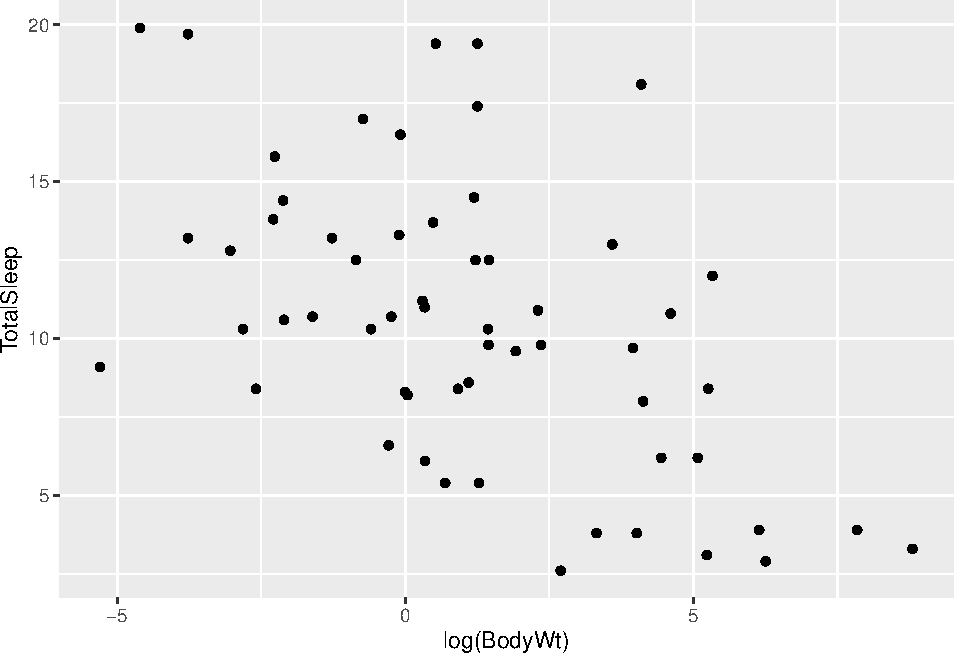
\includegraphics{DataScience_files/figure-latex/unnamed-chunk-21-1.pdf}

The ``Rotation'' matrix (fit{[}2{]}) contains the ``loadings'' of each of the original variables on the newly created PCs. Take a look at this matrix. The larger the absolute value of a variable in each PC, the more that variable contributes to that PC.

\hypertarget{biplots}{%
\subsection{Biplots}\label{biplots}}

We can use the function ``biplot'' to plot the first two PCs of our data. The plotted arrows provide a graphical rendition of the loadings of each of the original variables on the two PCs.

\begin{Shaded}
\begin{Highlighting}[]
\KeywordTok{biplot}\NormalTok{(fit)}
\end{Highlighting}
\end{Shaded}

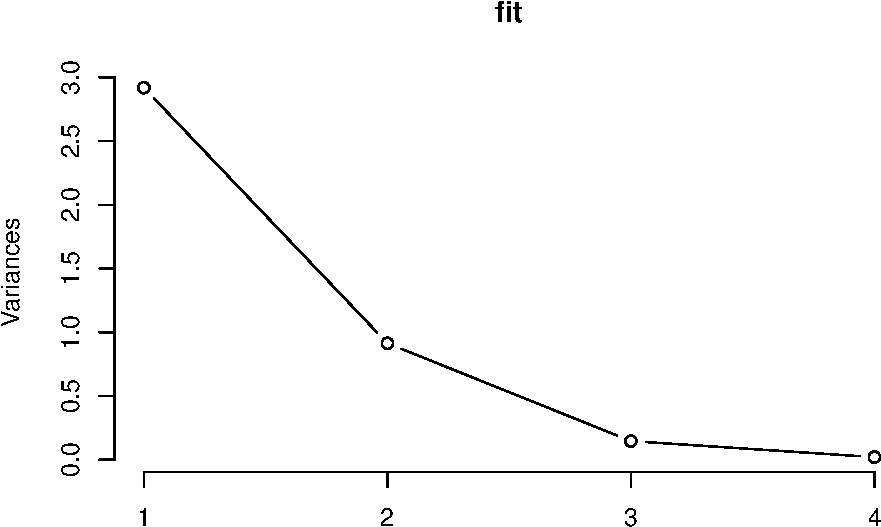
\includegraphics{DataScience_files/figure-latex/unnamed-chunk-22-1.pdf}

\hypertarget{exercise-2-interpreting-biplots}{%
\subsection{Exercise 2: Interpreting biplots}\label{exercise-2-interpreting-biplots}}

Across this reduced dimensional space, we can see that particular variables tend to co-vary quite strongly. Which ones? We can also see a separation into two groups on PC1. Which variables do you think would be most different between samples in one group and in the other?

\hypertarget{pca-using-ggplot}{%
\subsection{PCA using ggplot}\label{pca-using-ggplot}}

We can make prettier plots using ggplot2 and ggbiplot.

We first extract the variances of the principal components and then plot them:

\begin{Shaded}
\begin{Highlighting}[]
\NormalTok{variances \textless{}{-}}\StringTok{ }\KeywordTok{data.frame}\NormalTok{(}\DataTypeTok{variances=}\NormalTok{fit}\OperatorTok{$}\NormalTok{sdev}\OperatorTok{**}\DecValTok{2}\NormalTok{, }\DataTypeTok{pcomp=}\DecValTok{1}\OperatorTok{:}\KeywordTok{length}\NormalTok{(fit}\OperatorTok{$}\NormalTok{sdev))}
\NormalTok{varPlot \textless{}{-}}\StringTok{ }\KeywordTok{ggplot}\NormalTok{(variances, }\KeywordTok{aes}\NormalTok{(pcomp, variances)) }\OperatorTok{+}\StringTok{ }\KeywordTok{geom\_bar}\NormalTok{(}\DataTypeTok{stat=}\StringTok{"identity"}\NormalTok{, }\DataTypeTok{fill=}\StringTok{"gray"}\NormalTok{) }\OperatorTok{+}\StringTok{ }\KeywordTok{geom\_line}\NormalTok{()}
\NormalTok{varPlot}
\end{Highlighting}
\end{Shaded}

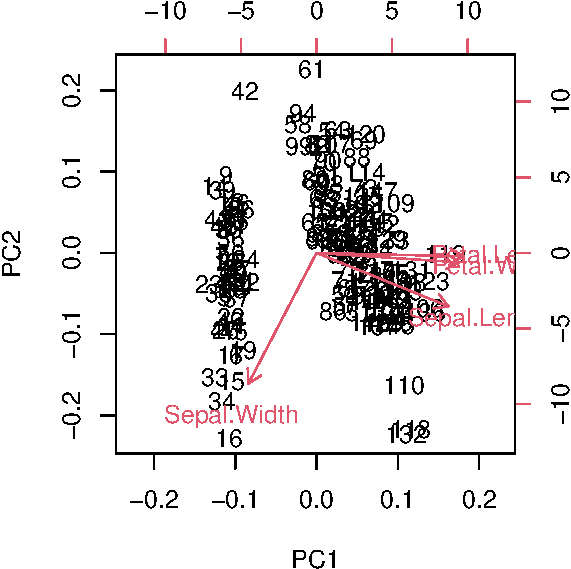
\includegraphics{DataScience_files/figure-latex/unnamed-chunk-23-1.pdf}

We can also plot the first two PCs, like we had done before in base R, but now coloring the samples by their corresponding species. How are the species distributed along PC1?

\begin{Shaded}
\begin{Highlighting}[]
\NormalTok{Species\textless{}{-}iris}\OperatorTok{$}\NormalTok{Species}
\NormalTok{iris\_pca \textless{}{-}}\StringTok{ }\KeywordTok{ggbiplot}\NormalTok{(fit,}\DataTypeTok{obs.scale =} \DecValTok{1}\NormalTok{, }
         \DataTypeTok{var.scale=}\DecValTok{1}\NormalTok{,}\DataTypeTok{groups=}\NormalTok{Species,}\DataTypeTok{ellipse=}\NormalTok{F,}\DataTypeTok{circle=}\NormalTok{F,}\DataTypeTok{varname.size=}\DecValTok{3}\NormalTok{)}
\NormalTok{iris\_pca}
\end{Highlighting}
\end{Shaded}

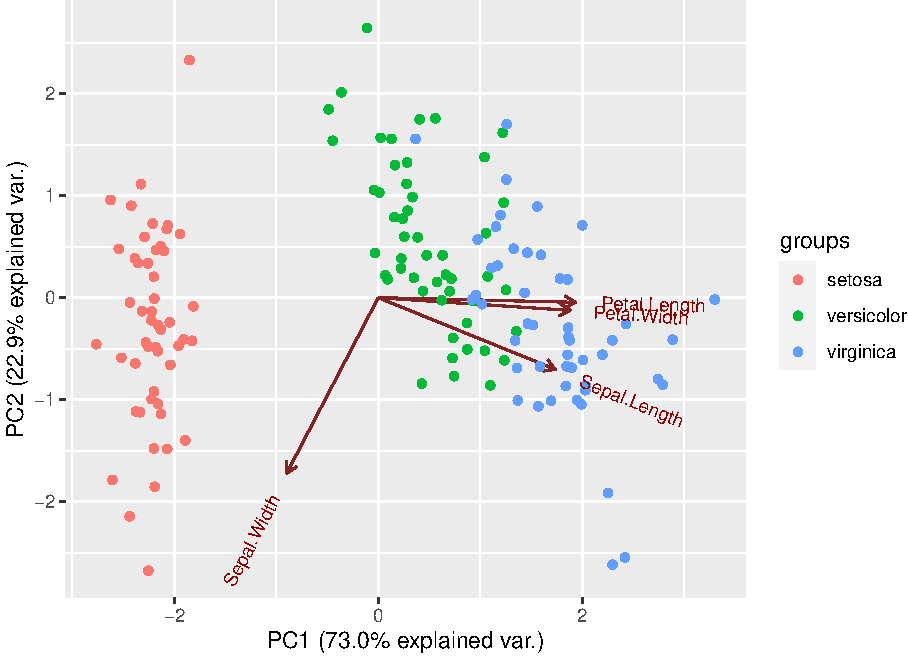
\includegraphics{DataScience_files/figure-latex/unnamed-chunk-24-1.pdf}

\hypertarget{pca-under-the-hood}{%
\subsection{PCA under the hood}\label{pca-under-the-hood}}

Rather than just using a ready-made function to compute a PCA, let's take a longer route to understand exactly what's happening under the hood of the prcomp() function.

First, let's standardize each column of our data so that each column has mean 0 and variance 1

\begin{Shaded}
\begin{Highlighting}[]
\NormalTok{irisdat \textless{}{-}}\StringTok{ }\NormalTok{iris[}\OperatorTok{{-}}\DecValTok{5}\NormalTok{]}
\NormalTok{irisstandard \textless{}{-}}\StringTok{ }\KeywordTok{apply}\NormalTok{(irisdat,}\DecValTok{2}\NormalTok{,}\ControlFlowTok{function}\NormalTok{(x)\{(x}\OperatorTok{{-}}\KeywordTok{mean}\NormalTok{(x))}\OperatorTok{/}\KeywordTok{sd}\NormalTok{(x)\})}
\end{Highlighting}
\end{Shaded}

Now, calculate the covariance matrix. Because the data has been standardized, this is equivalent to calculating the correlation matrix of the pre-standardized data.

\begin{Shaded}
\begin{Highlighting}[]
\NormalTok{cormat \textless{}{-}}\StringTok{ }\KeywordTok{cov}\NormalTok{(irisstandard)}
\end{Highlighting}
\end{Shaded}

Then, extract the eigenvalues and eigenvectors of correlation matrix:

\begin{Shaded}
\begin{Highlighting}[]
\NormalTok{myEig \textless{}{-}}\StringTok{ }\KeywordTok{eigen}\NormalTok{(cormat)}
\end{Highlighting}
\end{Shaded}

Now, we'll manually obtain certain values that were automatically computed by the prcomp function when we ran it earlier. We'll calculate the singular values (square root of eigenvalues) and also obtain the eigenvectors, also called loadings.

\begin{Shaded}
\begin{Highlighting}[]
\NormalTok{sdLONG \textless{}{-}}\StringTok{ }\KeywordTok{sqrt}\NormalTok{(myEig}\OperatorTok{$}\NormalTok{values)}
\NormalTok{loadingsLONG \textless{}{-}}\StringTok{ }\NormalTok{myEig}\OperatorTok{$}\NormalTok{vectors}
\KeywordTok{rownames}\NormalTok{(loadingsLONG) \textless{}{-}}\StringTok{ }\KeywordTok{colnames}\NormalTok{(irisstandard)}
\end{Highlighting}
\end{Shaded}

Using the loadings, we can plot our original (standardized) data matrix into the new PC-space, by multiplying the data matrix by the matrix of loadings. Plotting the first two rows of the resulting product should reveal the location of our data points in the first two principal components (like we had before):

\begin{Shaded}
\begin{Highlighting}[]
\NormalTok{scoresLONG \textless{}{-}}\StringTok{ }\NormalTok{irisstandard }\OperatorTok{\%*\%}\StringTok{ }\NormalTok{loadingsLONG}
\KeywordTok{plot}\NormalTok{(scoresLONG[,}\DecValTok{1}\NormalTok{],scoresLONG[,}\DecValTok{2}\NormalTok{])}
\end{Highlighting}
\end{Shaded}

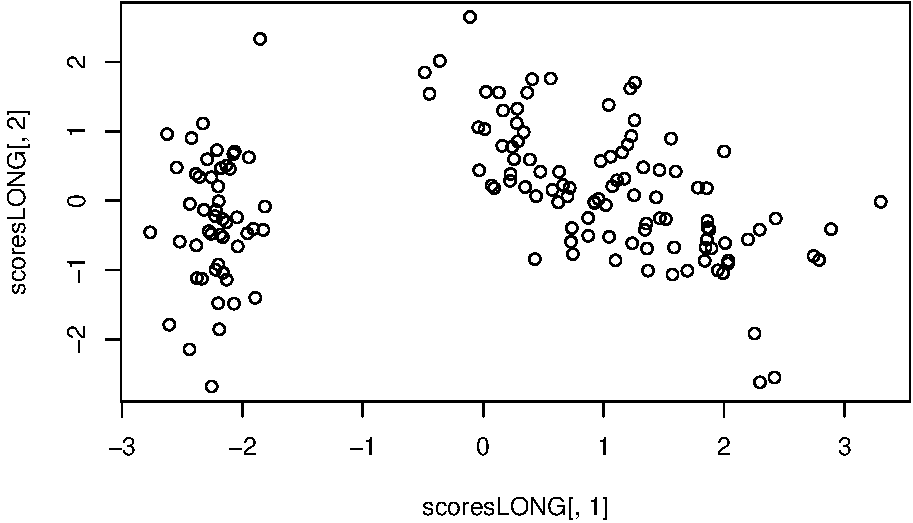
\includegraphics{DataScience_files/figure-latex/unnamed-chunk-29-1.pdf}

You can compare the results from the first section (using the ready-made function prcomp) and this section (taking a longer road), to check that the results are equivalent: the minimum and maximum differences in values for the loadings, the scores and standard deviations of the PCs are infinitesimally small.

\begin{Shaded}
\begin{Highlighting}[]
\KeywordTok{range}\NormalTok{(fit}\OperatorTok{$}\NormalTok{sdev }\OperatorTok{{-}}\StringTok{ }\NormalTok{sdLONG)}
\end{Highlighting}
\end{Shaded}

\begin{verbatim}
## [1] -2.775558e-16  6.661338e-16
\end{verbatim}

\begin{Shaded}
\begin{Highlighting}[]
\KeywordTok{range}\NormalTok{(fit}\OperatorTok{$}\NormalTok{rotation }\OperatorTok{{-}}\StringTok{ }\NormalTok{loadingsLONG)}
\end{Highlighting}
\end{Shaded}

\begin{verbatim}
## [1] -7.216450e-16  3.330669e-16
\end{verbatim}

\begin{Shaded}
\begin{Highlighting}[]
\KeywordTok{range}\NormalTok{(fit}\OperatorTok{$}\NormalTok{x }\OperatorTok{{-}}\StringTok{ }\NormalTok{scoresLONG) }
\end{Highlighting}
\end{Shaded}

\begin{verbatim}
## [1] -2.865763e-15  2.220446e-15
\end{verbatim}

\hypertarget{nmds}{%
\section{NMDS}\label{nmds}}

We'll now perform non-metric multidimensional scaling. Let's first take a look at the raw data we will use. This is a data matrix containing information about dune meadow vegetation. There are 30 species and 20 sites. Each cell corresponds to the number of specimens of a particular species that has been observed at a particular site (Jongman et al.~1987). As one can see, there are many sites where some species are completely absent (the cell value equals 0):

\begin{Shaded}
\begin{Highlighting}[]
\KeywordTok{data}\NormalTok{(dune)}
\NormalTok{dune}
\end{Highlighting}
\end{Shaded}

\begin{verbatim}
##    Achimill Agrostol Airaprae Alopgeni Anthodor Bellpere Bromhord Chenalbu
## 1         1        0        0        0        0        0        0        0
## 2         3        0        0        2        0        3        4        0
## 3         0        4        0        7        0        2        0        0
## 4         0        8        0        2        0        2        3        0
## 5         2        0        0        0        4        2        2        0
## 6         2        0        0        0        3        0        0        0
## 7         2        0        0        0        2        0        2        0
## 8         0        4        0        5        0        0        0        0
## 9         0        3        0        3        0        0        0        0
## 10        4        0        0        0        4        2        4        0
## 11        0        0        0        0        0        0        0        0
## 12        0        4        0        8        0        0        0        0
## 13        0        5        0        5        0        0        0        1
## 14        0        4        0        0        0        0        0        0
## 15        0        4        0        0        0        0        0        0
## 16        0        7        0        4        0        0        0        0
## 17        2        0        2        0        4        0        0        0
## 18        0        0        0        0        0        2        0        0
## 19        0        0        3        0        4        0        0        0
## 20        0        5        0        0        0        0        0        0
##    Cirsarve Comapalu Eleopalu Elymrepe Empenigr Hyporadi Juncarti Juncbufo
## 1         0        0        0        4        0        0        0        0
## 2         0        0        0        4        0        0        0        0
## 3         0        0        0        4        0        0        0        0
## 4         2        0        0        4        0        0        0        0
## 5         0        0        0        4        0        0        0        0
## 6         0        0        0        0        0        0        0        0
## 7         0        0        0        0        0        0        0        2
## 8         0        0        4        0        0        0        4        0
## 9         0        0        0        6        0        0        4        4
## 10        0        0        0        0        0        0        0        0
## 11        0        0        0        0        0        2        0        0
## 12        0        0        0        0        0        0        0        4
## 13        0        0        0        0        0        0        0        3
## 14        0        2        4        0        0        0        0        0
## 15        0        2        5        0        0        0        3        0
## 16        0        0        8        0        0        0        3        0
## 17        0        0        0        0        0        2        0        0
## 18        0        0        0        0        0        0        0        0
## 19        0        0        0        0        2        5        0        0
## 20        0        0        4        0        0        0        4        0
##    Lolipere Planlanc Poaprat Poatriv Ranuflam Rumeacet Sagiproc Salirepe
## 1         7        0       4       2        0        0        0        0
## 2         5        0       4       7        0        0        0        0
## 3         6        0       5       6        0        0        0        0
## 4         5        0       4       5        0        0        5        0
## 5         2        5       2       6        0        5        0        0
## 6         6        5       3       4        0        6        0        0
## 7         6        5       4       5        0        3        0        0
## 8         4        0       4       4        2        0        2        0
## 9         2        0       4       5        0        2        2        0
## 10        6        3       4       4        0        0        0        0
## 11        7        3       4       0        0        0        2        0
## 12        0        0       0       4        0        2        4        0
## 13        0        0       2       9        2        0        2        0
## 14        0        0       0       0        2        0        0        0
## 15        0        0       0       0        2        0        0        0
## 16        0        0       0       2        2        0        0        0
## 17        0        2       1       0        0        0        0        0
## 18        2        3       3       0        0        0        0        3
## 19        0        0       0       0        0        0        3        3
## 20        0        0       0       0        4        0        0        5
##    Scorautu Trifprat Trifrepe Vicilath Bracruta Callcusp
## 1         0        0        0        0        0        0
## 2         5        0        5        0        0        0
## 3         2        0        2        0        2        0
## 4         2        0        1        0        2        0
## 5         3        2        2        0        2        0
## 6         3        5        5        0        6        0
## 7         3        2        2        0        2        0
## 8         3        0        2        0        2        0
## 9         2        0        3        0        2        0
## 10        3        0        6        1        2        0
## 11        5        0        3        2        4        0
## 12        2        0        3        0        4        0
## 13        2        0        2        0        0        0
## 14        2        0        6        0        0        4
## 15        2        0        1        0        4        0
## 16        0        0        0        0        4        3
## 17        2        0        0        0        0        0
## 18        5        0        2        1        6        0
## 19        6        0        2        0        3        0
## 20        2        0        0        0        4        3
\end{verbatim}

Note that this data is non-linear, so our first instinct should not be to perform PCA on it. Because NMDS relies on ``distances'', we need to specify a distance metric that we'll use. The function for performing NMDS in the package `vegan' is called metaMDS() and its default distance metric is ``bray'', which corresponds to the Bray-Curtis dissimilarity: a statistic used to quantify the compositional dissimilarity between two different sites, based on counts at each site

Let's perform NMDS ordination using the Bray-Curtis dissimilarity. Remember that, unlike PCA, NMDS requires us to specify the number of dimensions (k) a priori (the default in vegan is 2). It also performs a series of transformations on the data that are appropriate for ecological data (default: autotransform=TRUE). The trymax option ensures that the algorithm is started from different points (in our case, 50) to avoid local minima.

\begin{Shaded}
\begin{Highlighting}[]
\NormalTok{ord \textless{}{-}}\StringTok{ }\KeywordTok{metaMDS}\NormalTok{(dune, }\DataTypeTok{k=}\DecValTok{2}\NormalTok{, }\DataTypeTok{autotransform =} \OtherTok{TRUE}\NormalTok{, }\DataTypeTok{trymax=}\DecValTok{50}\NormalTok{)}
\end{Highlighting}
\end{Shaded}

\begin{verbatim}
## Run 0 stress 0.1192678 
## Run 1 stress 0.1183186 
## ... New best solution
## ... Procrustes: rmse 0.02026472  max resid 0.06495728 
## Run 2 stress 0.1192678 
## Run 3 stress 0.1192678 
## Run 4 stress 0.1183186 
## ... New best solution
## ... Procrustes: rmse 3.494263e-05  max resid 0.0001200663 
## ... Similar to previous best
## Run 5 stress 0.1183186 
## ... Procrustes: rmse 2.012734e-05  max resid 6.950789e-05 
## ... Similar to previous best
## Run 6 stress 0.1192678 
## Run 7 stress 0.1808925 
## Run 8 stress 0.1922248 
## Run 9 stress 0.1192678 
## Run 10 stress 0.1183186 
## ... Procrustes: rmse 9.306821e-06  max resid 2.759834e-05 
## ... Similar to previous best
## Run 11 stress 0.1808911 
## Run 12 stress 0.1192679 
## Run 13 stress 0.1192678 
## Run 14 stress 0.1183187 
## ... Procrustes: rmse 9.901429e-05  max resid 0.0002953258 
## ... Similar to previous best
## Run 15 stress 0.1889656 
## Run 16 stress 0.1183186 
## ... Procrustes: rmse 5.050514e-06  max resid 1.603753e-05 
## ... Similar to previous best
## Run 17 stress 0.1183186 
## ... Procrustes: rmse 1.130636e-05  max resid 3.545251e-05 
## ... Similar to previous best
## Run 18 stress 0.1183186 
## ... Procrustes: rmse 4.297152e-06  max resid 7.616523e-06 
## ... Similar to previous best
## Run 19 stress 0.1192684 
## Run 20 stress 0.1183186 
## ... Procrustes: rmse 5.963945e-05  max resid 0.0001273425 
## ... Similar to previous best
## *** Solution reached
\end{verbatim}

As you can see, the function goes through a series of steps until convergence is reached. Let's plot the results:

\begin{Shaded}
\begin{Highlighting}[]
\KeywordTok{par}\NormalTok{(}\DataTypeTok{mfrow=}\KeywordTok{c}\NormalTok{(}\DecValTok{1}\NormalTok{,}\DecValTok{2}\NormalTok{))}
\KeywordTok{plot}\NormalTok{(ord,}\DataTypeTok{display=}\StringTok{"sites"}\NormalTok{,}\DataTypeTok{main=}\StringTok{"NMDS ordination of sites"}\NormalTok{,}\DataTypeTok{type=}\StringTok{"t"}\NormalTok{)}
\KeywordTok{plot}\NormalTok{(ord,}\DataTypeTok{display=}\StringTok{"species"}\NormalTok{,}\DataTypeTok{main=}\StringTok{"NMDS ordination of species"}\NormalTok{,}\DataTypeTok{type=}\StringTok{"t"}\NormalTok{)}
\end{Highlighting}
\end{Shaded}

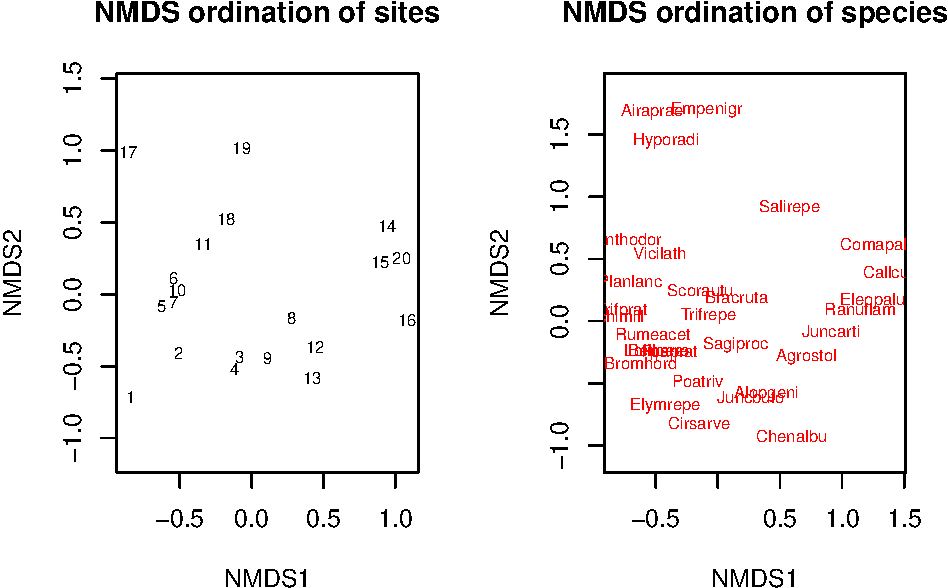
\includegraphics{DataScience_files/figure-latex/unnamed-chunk-33-1.pdf}

\begin{Shaded}
\begin{Highlighting}[]
\KeywordTok{par}\NormalTok{(}\DataTypeTok{mfrow=}\KeywordTok{c}\NormalTok{(}\DecValTok{1}\NormalTok{,}\DecValTok{1}\NormalTok{))}
\end{Highlighting}
\end{Shaded}

\hypertarget{exercise-3-interpreting-nmds-plots}{%
\subsection{Exercise 3: interpreting NMDS plots}\label{exercise-3-interpreting-nmds-plots}}

What do these plots tell you about the distribution of species across sites? Which species tend to co-occcur with each other? Which sites tend to have similar species compositions?

Try changing the number of dimensions or the distance metric used. You can take a look at the list of possible distances and their definitions using ``?vegdist''. Do the results change? Why?

  \bibliography{book.bib,packages.bib}

\end{document}
